\documentclass[a4paper,10pt]{article}
\usepackage[brazilian]{babel}
\usepackage[left=2.5cm,right=2.5cm,top=3cm,bottom=2.5cm]{geometry}
\usepackage{mathtools}
\usepackage{amsthm}
\usepackage{amsmath}
%\usepackage{nccmath}
\usepackage{amssymb}
\usepackage{amsfonts}
\usepackage{physics}
%\usepackage{dsfont}
%\usepackage{mathrsfs}

\usepackage{titling}
\usepackage{indentfirst}

\usepackage{bm}
\usepackage[dvipsnames]{xcolor}
\usepackage{cancel}

\usepackage{xurl}
\usepackage[colorlinks=true]{hyperref}

\usepackage{float}
\usepackage{graphicx}
%\usepackage{tikz}
\usepackage{caption}
\usepackage{subcaption}

%%%%%%%%%%%%%%%%%%%%%%%%%%%%%%%%%%%%%%%%%%%%%%%%%%%

\newcommand{\eps}{\epsilon}
\newcommand{\vphi}{\varphi}
\newcommand{\cte}{\text{cte}}

\newcommand{\N}{\mathbb{N}}
\newcommand{\Z}{\mathbb{Z}}
\newcommand{\Q}{\mathbb{Q}}
\newcommand{\R}{\vb{R}}
\newcommand{\C}{\mathbb{C}}
\renewcommand{\S}{\hat{S}}
%\renewcommand{\H}{\s{H}}

\renewcommand{\a}{\vb{a}}
\newcommand{\nn}{\hat{n}}
\renewcommand{\d}{\dagger}
\newcommand{\up}{\uparrow}
\newcommand{\down}{\downarrow}

\newcommand{\0}{\vb{0}}
%\newcommand{\1}{\mathds{1}}
\newcommand{\E}{\vb{E}}
\newcommand{\B}{\vb{B}}
\renewcommand{\v}{\vb{v}}
\renewcommand{\r}{\vb{r}}
\renewcommand{\k}{\vb{k}}
\newcommand{\p}{\vb{p}}
\newcommand{\q}{\vb{q}}
\newcommand{\F}{\vb{F}}

\newcommand{\s}{\sigma}
%\newcommand{\prodint}[2]{\left\langle #1 , #2 \right\rangle}
\newcommand{\cc}[1]{\overline{#1}}
\newcommand{\Eval}[3]{\eval{\left( #1 \right)}_{#2}^{#3}}

\newcommand{\unit}[1]{\; \mathrm{#1}}

\newcommand{\n}{\medskip}
\newcommand{\e}{\quad \mathrm{e} \quad}
\newcommand{\ou}{\quad \mathrm{ou} \quad}
\newcommand{\virg}{\, , \;}
\newcommand{\ptodo}{\forall \,}
\renewcommand{\implies}{\; \Rightarrow \;}
%\newcommand{\eqname}[1]{\tag*{#1}} % Tag equation with name

\setlength{\droptitle}{-7em}

\theoremstyle{plain}
\newtheorem{theorem}{Teorema}[section]
%\newtheorem{defi}[theorem]{Definição}
\newtheorem{lemma}[theorem]{Lema}
%\newtheorem{corol}[theorem]{Corolário}
%\newtheorem{prop}[theorem]{Proposição}
%\newtheorem{example}{Exemplo}
%
%\newtheorem{inneraxiom}{Axioma}
%\newenvironment{axioma}[1]
%  {\renewcommand\theinneraxiom{#1}\inneraxiom}
%  {\endinneraxiom}
%
%\newtheorem{innerpostulado}{Postulado}
%\newenvironment{postulado}[1]
%  {\renewcommand\theinnerpostulado{#1}\innerpostulado}
%  {\endinnerpostulado}
%
%\newtheorem{innerexercise}{Exercício}
%\newenvironment{exercise}[1]
%  {\renewcommand\theinnerexercise{#1}\innerexercise}
%  {\endinnerexercise}
%
%\newtheorem{innerthm}{Teorema}
%\newenvironment{teorema}[1]
%  {\renewcommand\theinnerthm{#1}\innerthm}
%  {\endinnerthm}
%
\newtheorem{innerlema}{Lema}
\newenvironment{lema}[1]
  {\renewcommand\theinnerlema{#1}\innerlema}
  {\endinnerlema}
%
%\theoremstyle{remark}
%\newtheorem*{hint}{Dica}
%\newtheorem*{notation}{Notação}
%\newtheorem*{obs}{Observação}


\usepackage[shortlabels]{enumitem}

\title{\Huge{\textbf{Fuja do Nabo - P2}}}
\date{\vspace{-10ex}}

\begin{document}

\maketitle

\subsection*{1. Questões 7-10 da P1 de 2022}

Um corpo preso na extremidade de uma mola e imerso em um
fluido viscoso, executa um movimento harmônico amortecido no regime subcrítico conforme a equação
horária:
$$
x(t) = 4 e^{-3t} \cos(4t + \phi) \unit{m}.
$$
O corpo tem massa $M=1 \unit{kg}$ e possui velocidade nula no instante de tempo $t = 0 \unit{s}$. Sabendo que
a equação diferencial deste movimento é
$$
\ddot{x} + \gamma \dot{x} + \omega_0^2x = 0.
$$
Determine:

\begin{enumerate}[(a)]
\item A frequência natural de oscilação $\omega_0$ e a constante de viscosidade $b = \gamma M$.

\item A fase inicial $\phi$ do movimento.

\item O tempo necessário para que a amplitude máxima do movimento se reduza à metade do valor inicial.

\item Supondo que seja possível variar apenas $\gamma$, qual deveria ser seu valor para o caso
do amortecimento crítico? Da mesma forma, supondo que seja possível variar apenas $\omega_0$, qual
deveria ser seu valor para o caso do amortecimento supercrítico?
\end{enumerate}

\n\n\n

\subsection*{2. Questões 1-3 da P2 de 2022}

Um bloco de massa $m = 2 \unit{kg}$, preso a duas molas idênticas, com
comprimentos naturais iguais a $l_0 = 0.5 \unit{m}$ e constantes elásticas iguais a $k = 400 \unit{N/m}$, estão dentro
de um recipiente com um líquido, cujo coeficiente de atrito viscoso vale $b = 80 \unit{kg/s}$. Uma força
harmônica de amplitude $F_0 = 100 \unit{N}$ e frequência angular $\Omega = 10 \unit{rad/s}$ atua sobre o bloco ao
longo da direção horizontal. O atrito entre o bloco e o fundo do recipiente é desprezível. Usando o
referencial da figura, determine:
\begin{figure}[H]
\centering
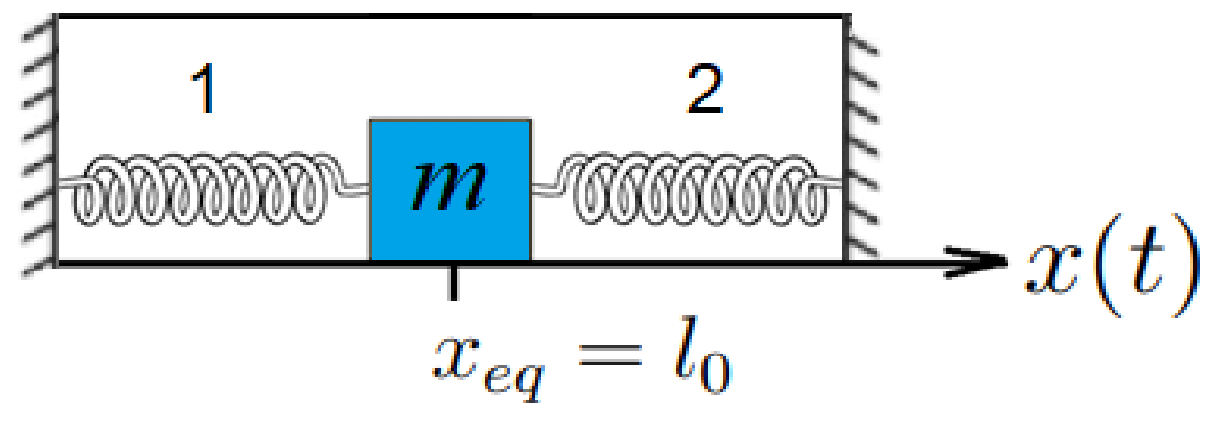
\includegraphics[width=0.9\linewidth]{fig/duas_molas.png}
\label{fig:duas_molas}
\end{figure}

Determine:
\begin{enumerate}[(a)]
\item A expressão da força elástica que as molas exercem sobre o corpo.

\item A frequência natural de oscilação $\omega_0$.

\item A solução da equação de movimento no regime estacionário, em função de $t$,
considerando $x_{\text{eq}}=0 \unit{m}$.
\end{enumerate}


\subsection*{3. Questões 1-3 da REC de 2022}

O gráfico de $x(t)$, mostrado na figura abaixo, representa a equação
horária de um oscilador criticamente amortecido, para um sistema composto de um corpo de massa
$m = 1 \unit{kg}$ preso a uma mola de constante elástica $k$ e imerso em um líquido viscoso, de coeficiente
de resistência viscosa $b$. A equação horária pode ser escrita como $x(t) = e^{-\frac{\gamma}{2} t} (A + Bt)$.
\begin{figure}[H]
\centering
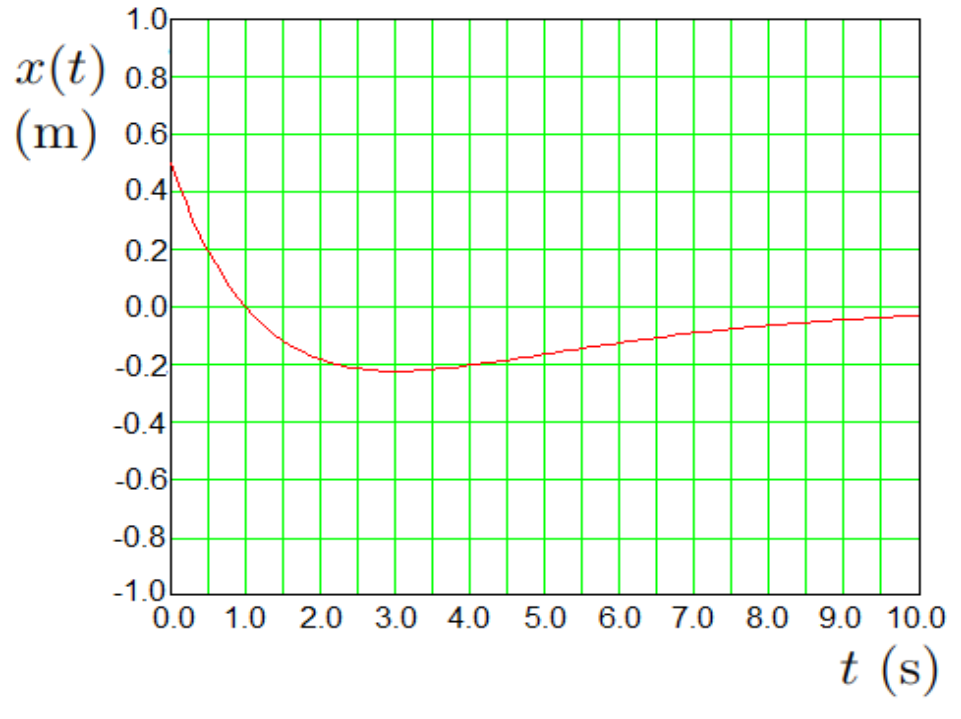
\includegraphics[width=0.9\linewidth]{fig/grafico_rec.png}
\label{fig:grafico_rec}
\end{figure}

\begin{enumerate}[(a)]
\item Determine os valores de $A$ e $B$.

\item Determine o coeficiente de resistência viscosa $b$ e a constante elástica $k$ da mola.

\item Determine o valor da velocidade inicial $v_0$ do oscilador.
\end{enumerate}

\n

\subsection*{4. Questão 2 da 2\textsuperscript{\underline{a}} da Lista de Exercícios}

Um corpo de massa $m$ desliza sobre um plano horizontal sem atrito sujeito a três
forças: uma força elástica resultante da ação de uma mola de constante elástica
$k$, uma força devido à resistência viscosa do meio, caracterizada pela constante de
resistência viscosa $b$ e uma força externa periódica $F(t) = F_0 \cos(\Omega t)$, sendo $\Omega$ a
frequência externa.

\begin{enumerate}[(a)]
\item Escreva a equação diferencial que descreve o movimento do corpo e encontre a
sua solução estacionária.

\item Considerando que $m = 50 \unit{kg}$, $k = 5000 \unit{N/m}$, $F_0 = 50 \unit{N}$ e $b = 500 \unit{kg/s}$, calcule
a frequência natural do sistema e o seu fator de qualidade $Q$.

\item No regime estacionário, usando os valores do item anterior, determine o valor
de $\Omega$ para o qual a amplitude $A$ do movimento é máxima.

\item No regime estacionário, usando os valores do item (b), determine o valor da
amplitude máxima.
\end{enumerate}

\n

\subsection*{5. Questões 2-5 da SUB de 2022}

O gráfico abaixo representa a equação horária $x(t)$ de um oscilador,
para um sistema composto por um bloco de massa $m = 1 \unit{kg}$ preso a uma mola de constante elástica
$k$ que está na posição horizontal. Este sistema está imerso em um líquido viscoso com coeficiente
de resistência $b = 0.4 \unit{Ns/m}$ e cuja força de resistência é proporcional à velocidade do corpo que se
movimenta em seu interior. Dado que a velocidade inicial do bloco é $v_0 = −2 \unit{m/s}$, considerando o
intervalo de tempo mostrado no gráfico, responda:

\begin{figure}[H]
\centering
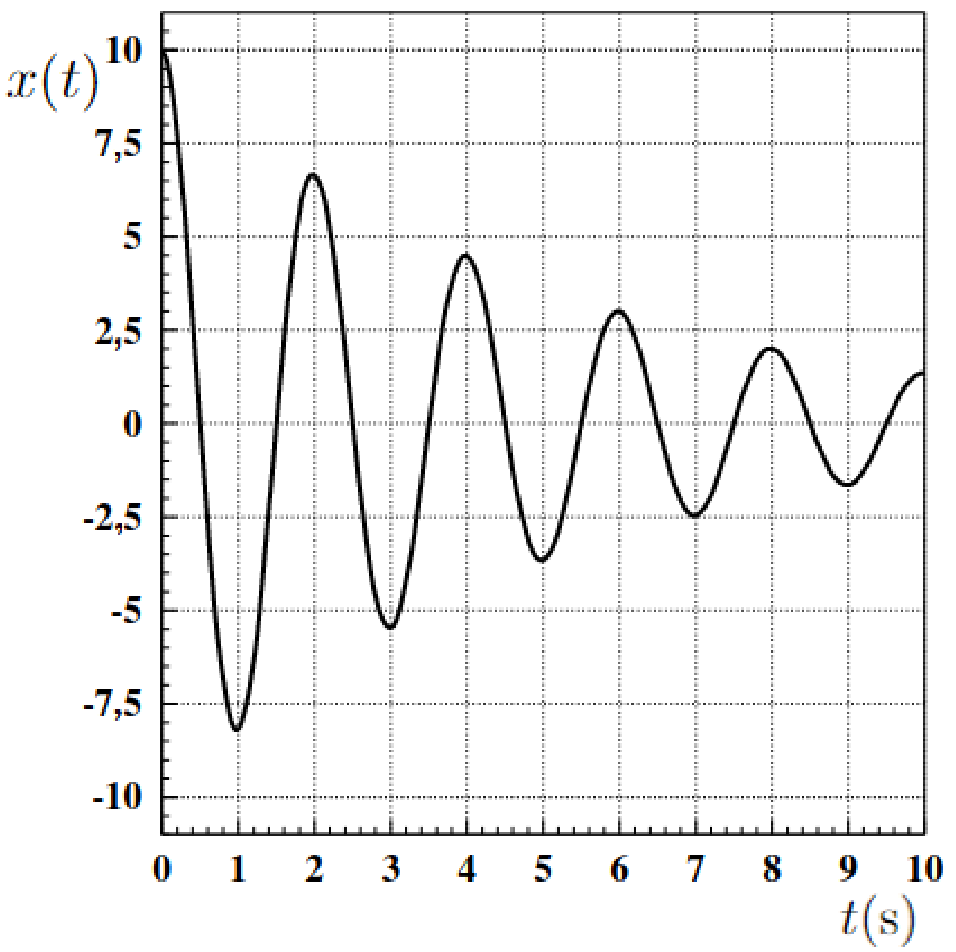
\includegraphics[width=0.8\linewidth]{fig/grafico_sub}
\label{fig:grafico_sub}
\end{figure}

\begin{enumerate}[(a)]
\item Dado o movimento do bloco no sistema descrito acima, qual a equação horária que
descreve este sistema?

\item Determine a constante elástica da mola $k$.

\item Qual a velocidade do bloco no instante $t = 3 \unit{s}$?

\item Suponha agora que este mesmo sistema seja retirado do líquido viscoso e passe a
oscilar num meio sem resistência. Neste novo regime, o deslocamento máximo é $x_{\text{max}}=10 \unit{m}$ e a
constante de fase é nula. Qual será a nova equação horária do sistema?
\end{enumerate}

\n

\subsection*{6. Questão 5 da REC de 2022}

Um oscilador unidimensional não amortecido, de massa $m = 0.50 \unit{kg}$ e frequência
própria $\omega_0 = 2.0 \unit{s^{-1}}$, move-se sobre um plano horizontal sob a ação de uma força externa não
periódica $F(t) = F_0 e^{-\beta t}$, com $F_0 = 40 \unit{N}$ e $\beta = 6.0 \unit{s^{-1}}$. Inicialmente o oscilador
encontra-se em repouso na posição de equilíbrio. Lembrando que a solução de uma equação diferencial não homogênea
é igual à solução da homogênea somada à solução particular (equação completa), determine a função
$x(t)$ que descreve o movimento do oscilador, com as condições iniciais acima.

\pagebreak

\section*{Gabarito}

\subsection*{1}

\begin{enumerate}[(a)]
\item $\omega_0 = 5 \unit{rad/s}$; $b = 6 \unit{kg/s}$.

\item $\phi = \arctan(-\frac{3}{4})$.

\item $t = \frac{\ln(2)}{3}$.

\item $\gamma = 10 \unit{s^{-1}}$; $\omega_0 < 3 \unit{rad/s}$.
\end{enumerate}

\subsection*{2}

\begin{enumerate}[(a)]
\item $F = -2k(x-l_0)$.

\item $\omega_0 = 20 \unit{rad/s}$.

\item $x(t) = 0.1 \cos[10t - \arctan(4/3)] \unit{m}$.
\end{enumerate}

\subsection*{3}

\begin{enumerate}[(a)]
\item $A = 0.5 \unit{m}$ e $B = -0.5 \unit{m/s}$.

\item $b = 1 \unit{kg/s}$ e $k = 0.25 \unit{N/m}$.

\item $v_0 = -0.75 \unit{m/s}$.
\end{enumerate}


\subsection*{4}

\begin{enumerate}[(a)]
\item $\ddot{x} + \gamma \dot{x} + \omega_0^2 x = \frac{F_0}{m} \cos(\Omega t)$;
$x(t) = A(\Omega) \cos(\Omega t + \phi(\Omega))$, com
$$
A(\Omega) = \frac{F_0}{m \sqrt{(\omega_0^2-\Omega^2)^2 + \gamma^2\Omega^2}}
\e
\phi(\Omega) = - \arctan(\frac{\gamma \Omega}{\omega_0^2 - \Omega^2}).
$$

\item $\omega_0 = 10 \unit{s^{-1}}$, $Q = 1$.

\item $\Omega_{\text{max}} = 5\sqrt{2} \unit{s^{-1}}$.

\item $A_{\text{max}} = \frac{1}{50\sqrt{3}} \unit{m}$.
\end{enumerate}


\subsection*{5}

\begin{enumerate}[(a)]
\item $x(t) = 10 e^{-0.2 t} \cos(\pi t) \unit{m}$.

\item $k = (\pi^2 + 0.04) \unit{kg/s^2}$.

\item $v(t = 3 \unit{s}) = 2 \, e^{-0.6} \unit{m/s}$.

\item $x(t) = 10 \cos(\sqrt{\pi^2 + 0.04} \, t) \unit{m}$.
\end{enumerate}

\subsection*{6}

\begin{enumerate}[(a)]
\item $x(t) = 2 \qty[e^{-6t} - \cos(2t) + 3 \sin(2t)] \unit{m}$.
\end{enumerate}

\end{document}
